%----------------------------------------------------------------------------------------
%	PACKAGES AND OTHER DOCUMENT CONFIGURATIONS
%----------------------------------------------------------------------------------------

\documentclass[12pt]{article}
\usepackage{graphicx}
\usepackage[utf8]{inputenc}  
\usepackage[T1]{fontenc} 
\usepackage[top=2cm,bottom=2cm,left=1.3cm,right=1.5cm,asymmetric]{geometry}
\usepackage{amsfonts}
\usepackage{graphicx}
\usepackage{caption}
\usepackage{subcaption}
\usepackage{float}
\usepackage{subfig}
\usepackage{algorithm}
\usepackage{algpseudocode}
\usepackage{fancyhdr}
\usepackage{ stmaryrd }
\usepackage{placeins}
\usepackage{ amssymb }
\usepackage{mathtools}
\pagestyle{fancy}
\renewcommand{\footrulewidth}{1pt}
\fancyhead[R]{\textit{Master MVA : Reinforcement Learning}}
\fancyfoot[L]{\textit{}}
%\usepackage{unicode-math}
%\setmathfont{XITS Math}
%\setmathfont[version=setB,StylisticSet=1]{XITS Math}
\usepackage{array,multirow,makecell}
\setcellgapes{1pt}
\makegapedcells
\newcolumntype{R}[1]{>{\raggedleft\arraybackslash }b{#1}}
\newcolumntype{L}[1]{>{\raggedright\arraybackslash }b{#1}}
\newcolumntype{C}[1]{>{\centering\arraybackslash }b{#1}}

\pagestyle{fancy}
\renewcommand{\footrulewidth}{1pt}
\fancyfoot[L]{\textit{}}
   

\begin{document}
\begin{center}
\section*{Final project}
\section*{One algorithm for both stochastic and adversarial bandits}
\large{Izabella Joanna Lukasewitz \& Sammy Khalife}
\end{center}

\section*{Introduction}
In the multiarmed bandit game we will suppose here that the rewards (or losses, by changing the sign), are generated independently of the considered algorithms. If $r_{s}^{A_{s}}$ is the reward obtained at time s by pulling arm $A_{s}$, the regret is defined in the general framework as :
$$R(t)=\max_{a}\{ \sum_{s=1}^{t} \mathbb{E}[r_{s}^{a}]\}-\sum_{s=1}^{t} \mathbb{E}[r_{s}^{A_{s}}]$$~\\
In the \textbf{adversarial regime}, the losses are generated by a ''unrestricted adversary'' (knowing all the algorithm's actions). This can be seen as playing against an adversary in a two-players zero sum game, where the adversary has full information about the game.~\\
~\\
In the \textbf{stochastic regime}, we suppose that the rewards are sampled with a distribution independent from time, then $\mathbb{E}[r_{s}^{a}]=\mu_{a}$, and the regret simplifies : 
$$R(t)=t\max_{a}\mu_{a}-\sum_{s=1}^{t} \mathbb{E}[r_{s}^{A_{s}}]$$
which can be written $$R(t)=\sum_{a}\mathbb{E}[N_{t}(a)]\Delta_{a}$$ where $\Delta(a)=(\max_{a'}\mu_{a'})-\mu_{a}$ and $N_{t}(a)$ is the number of time a has been pulled until time t.
The aim of this part is to present an algorithm which garantees a logarithmic regret in both adversarial and stochastic framework.~\\
~\\
We can introduce 2 more frameworks for multiarmed bandit.~\\
~\\
The first of them is called \textbf{adversarial regime with a gap}, which is an adversarial regime for which we suppose that there exists a round $\tau$ and an arm $a_{\tau}*$ such that for any $t \geq \tau$, $a_{\tau}*$ persists to be the best arm in hindsight for all rounds $t \geq \tau$, i.e $\forall t \geq \tau a_{\tau}* \in argmin_{a'}(\sum_{s=1}^{t}l_{s}^{a'})$~\\
~\\
The \textbf{contamined stochastic regime} is a mix between stochastic regime and adversarial regime, where the adversary picks up some pairs $(t,a)$ (''locations'') before the game starts and assigns the rewards in an arbitrary way. The rest of the rewards are generated as in the stochastic framework.
\newpage
\section*{An adaptated EXP3 algorithm}

As a reminder, the EXP3 algorithm is made as follows : 
\FloatBarrier
\begin{algorithm}
\caption{EXP3}\label{RS}
Given fixed exploitation parameter $\eta$ and exploration parameter $\beta$\\
$\forall$ a $\omega_{a}(1)=1$\\
1. for t=2:$T_{end}$\\
2. $p_{a}(t) = (1-\beta)\frac{\omega_{a}(t-1)}{\sum_{a}\omega_{a}(t-1)}+\frac{\beta}{K}$\\
3. $A_{t}$ drawn with $p_{a}(t)$ distribution on arms\\
4. $\tilde{r}_{A_{t}} = \frac{r_{A_{t}}}{p_{A_{t}}(t-1)}$ and update of $\omega$ on $A_{t}$ only : $\omega_{A_{t}}(t)=\omega_{A_{t}}(t-1)exp(\eta \tilde{r}_{A_{t}(t)})$\\
\end{algorithm}
\FloatBarrier
~\\
The EXP3 algorithm (Auer et al., 2002) is very efficient for adversarial frameworks, but has some difficulties to adapt to every kind of problems. Below the regrets in a stochastic framework compared with one of the most efficient algorithm in this case (Thompson sampling) :
\begin{center} \textbf{Comparaison of Thompson and EXP3 on stochastic framework}\end{center}
 \begin{figure}[!h]
   \begin{minipage}[c]{0.5 \linewidth}
   \centering
    \captionsetup{justification=centering,margin=1cm}
      \includegraphics[width=9cm]{Thompson_vs_exp3.jpg}
      \caption{''Easy problem''\\KL complexity = 6.3 (6 arms) $\beta=0.01$, $\eta$=0.01}
   \end{minipage} \hfill
   \begin{minipage}[c]{0.5 \linewidth}
   \centering
   \captionsetup{justification=centering,margin=1cm}
      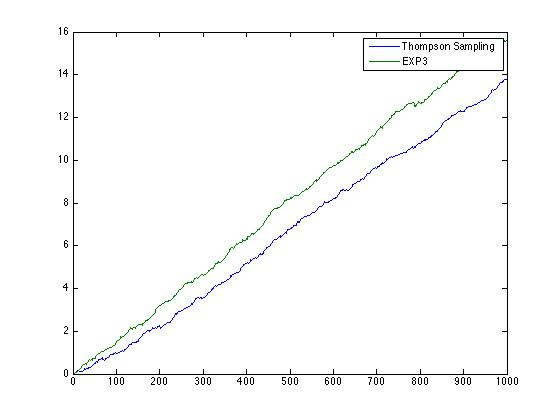
\includegraphics[width=9cm]{complexPbVs.jpg}
      \caption{''Difficult problem'',\\KL complexity = 315 (10 arms) $\beta$=0.01, $\eta$=0.01}
   \end{minipage} 
\end{figure}
~\\
To adapt EXP3 to stochastic configurations, the idea of the algorithm named EXP3++ (cf [1]) is to replace the exploration parameter $\beta$ and exploitation parameter $\eta$ by new time-depending parameters.
~\\
\FloatBarrier
\begin{algorithm}
\caption{EXP3++}\label{RS}
$\forall$ a $\tilde{L}_{0}(a)=0$\\
1. for $t=1:T_{end}$~\\
2. $\forall$ a $\in \{1,..K\}$\\
 $\epsilon_{t}(a)=min\{\frac{1}{2K}, \beta_{t}, \xi_{t}(a)\}$ \\
$\rho_{t}(a)=exp(-\eta_{t}\tilde{L}_{t-1}(a))/\sum_{a'}exp(-\eta_{t}\tilde{L}_{t-1}(a'))$\\
$\tilde{\rho}_{t}(a)=(1-\sum_{a'}\epsilon_{t}(a'))\rho_{t}(a)+\epsilon_{t}(a)$\\
3. Draw action $A_{t}$ with the $\tilde{\rho}_{t}$ distribution on arms.~\\
4. Observe the loss $l_{t}^{A_{t}}$ and $\forall$ a $\in \{1,..,K\}$\\
$\tilde{l}_{t}^{a}=\frac{l_{t}^{A_{t}}}{\tilde{\rho}_{t}(a)} \textbf{1}_{A_{t}=a}$\\
$\tilde{L}_{t}(a)=\tilde{L}_{t-1}(a)+\tilde{l}_{t}^{a}$
\end{algorithm}
\FloatBarrier~\\
With $\eta_{t}=2\beta_{t}$ and $\xi_{t}(a)=0$ we find back EXP3.
\section*{Theoretical results for EXP3++}
The main results have been demonstrated by Seldin and Slivkins [1]. 
\subsection*{Adversarial regimes}
~\\
\textbf{Theorem 1} For $\eta_{t}=\beta_{t}$ and $\xi(t) \geq 0$, the regret for any $t\geq0$ satisfies $$R(t) \leq 4\sqrt{K\ln K}$$ This upper bound is two times above the EXP3 theoretical upper bound.~\\
~\\
\subsection*{Stochastic regime}
First, if one supposes that we know the gaps, EXP3++ allows by defining adapted $\xi_{t}$ and $\eta_{t}$ to control the regret. In practice the gaps are not known and one will use an emprirical estimator : $$\hat{\Delta}_{t}(a)=min\{1,\frac{1}{t}(\max_{a'}(\tilde{L}_{t}(a')-\tilde{L}_{t}(a))\}$$
\textbf{Theorem 2} Knowing the gaps $\Delta(a)$, with $\xi_{t}(a)=\frac{c\ln(t\Delta(a)^{2})}{t\Delta(a)^{2}}$, the regret satisfies :
$$R(t) \leq \sum_{a} O(\frac{\ln(t)^{2}}{\Delta(a)})+\sum_{a}\tilde{O}(\frac{K}{\Delta(a)^{3}})$$
~\\
\textbf{Theorem 3} Let us consider the empirical gap $\Delta_{t}(a)$ defined previously, a time $t^{*}$ such that $t^{*}\geq \frac{4c^{2}K\ln(t*)^{4}}{\ln(K)}$ and let $t^{*}(a)=max\{t*,\lceil e^{1/\Delta(a)^{2}}\rceil\}$.
Then by tuning $\xi_{t}(a)=\frac{c\ln(t)^{2}}{t\hat{\Delta}_{t-1}(a)^{2}}$ (giving the EXP3$++^{AVG}$ algorithm) the regret in the stochastic regime satisfies :
$$R(t) \leq \sum_{a}O(\frac{\ln(t)^{3}}{\Delta{a}})+\sum_{a}\Delta(a)t^{*}(a)$$
\subsection*{Contamined stochastic regime}
\textbf{Theorem 4} With the same assumptions as theorem 3 except $t^{*}(a)=max\{t^{*}, \lceil e^{4/\Delta(a)^{2}}\rceil \}$, the regret satisfies :
$$R(t) \leq \sum_{a}O(\frac{\ln(t)^{3}}{\Delta(a)})+\sum_{a}max\{t^{*}(a),\tau\}$$
\subsection*{Adversarial regime with a gap}
\textbf{Theorem 5} With the same assumptions as in theorem 3, the regret satisfies :
$$R(t) \leq \sum_{a}\{\min_{\tau}\{max\{t^{*},\tau,e^{1/(\Delta(\tau,a))^{2}}\}+O(\frac{\ln(t)^{3}}{\Delta(\tau,a)})\}$$~\\
~\\
With $\eta_{t}=\beta_{t}$, the EXP3++ algorithm provides a guarantee against adversarial situations. On the other hand, a configuration such that $\eta=1$ provide better results on a stochastic configuration. Still a lot has to be done concerning this trade-off.
\section*{Numerical comparaison}

\section*{References}
$[1]$ One practical algorithm for both stochastic and adversarial bandits, Yevgeny Seldin, Queenslan University of Technology, Brisbane \& Aleksandrs Slivkins, Microsoft Research, New York~\\
~\\
$[2]$
\end{document}